%
%
\documentclass[10pt]{article}
%\usepackage[latin1]{inputenc}
\usepackage{amsmath}
%\usepackage{amsfonts}
\usepackage{amssymb}
\usepackage{graphicx}
\usepackage{hyperref}
\usepackage{booktabs}
\usepackage{multirow}
\usepackage{hhline}
\usepackage{vmargin}



%%%%%%%%%%%%%%%%%%%%%%%%%%%%%%
\title{The Advanced LIGO Input Mode Cleaner}
\author{Chris Mueller}
%\ligodraft
%%%%%%%%%%%%%%%%%%%%%%%%%%%%%%%%%%%%%%%%%%%%%%%%%%%%%%%%%%%%%%%%%%%%%
\begin{document}

%%%%%%%%%%%%%%%%%%%%%%%%%%%%%%%%%%%%%%%%%%%%%%%%%%%%%%%%%%%%%%%%
\begin{large}
\begin{center}
\begin{LARGE}
\textbf{The Advanced LIGO Input Mode Cleaner}\\
\end{LARGE}
\vspace{0.50in}
\textbf{Chris Mueller} \\
Dept. of Physics, University of Florida\\
\today
\end{center}
\end{large}
\vspace{1pc}
\tableofcontents
\pagebreak[4]

%==================================================================================================
\section{Input Mode Cleaner}

The input mode cleaner is the heart of the input optics, serving simultaneously as a spatial filter, 
polarization filter, frequency reference, and pointing reference.  
It is an in-vacuum, suspended, three mirror cavity with the mirrors hanging from the LIGO small triple 
suspensions \textbf{citation}.  
It has a free spectral range of 9.099 MHz and a finesse of 515.  
The beam is injected along one of the long arms and extracted along the other (see \ref{fig:ioAll}).  
The reflected beam is outfitted with an RF photodiode for Pound-Drever-Hall length sensing \textbf{citation} 
and two wavefront sensors for angular control.  
In addition, a pickoff of the intra-cavity light is extracted behind the curved mirror, MC2, and sent to a 
quadrant photodiode for additional angular information.  

\begin{figure}
	\centering
	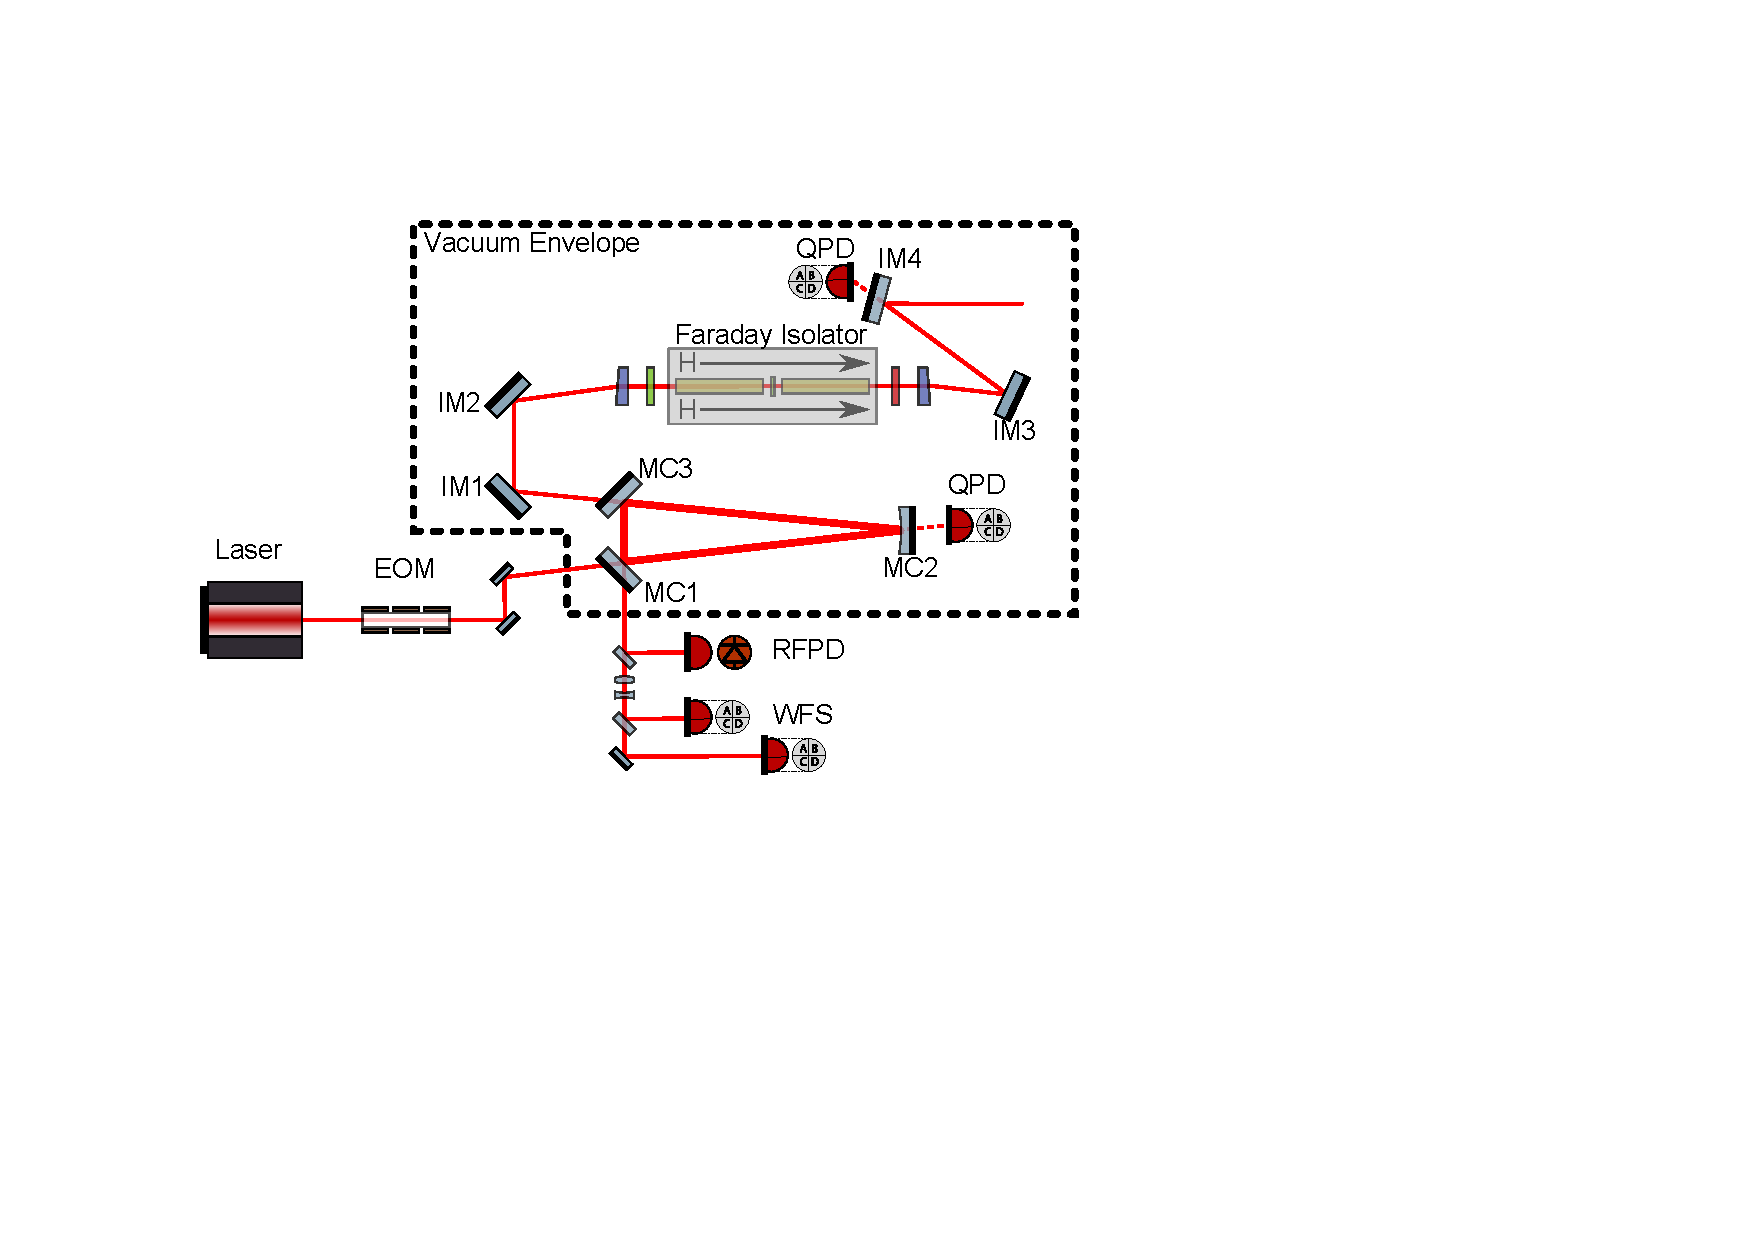
\includegraphics[width=0.9\textwidth, trim=3.5cm 7.5cm 11cm 3.5cm]{IO_Drawing.pdf}
	\caption{A schematic layout of the input optics is shown.  
		The input mode cleaner is represented by the three mirrors MC1, MC2, and MC3.  
		It is an in vacuum triply suspended triangular cavity used as a frequency 
		and pointing reference.  It also passively filters the spatial structure 
		and polarization of the incoming beam.}
	\label{fig:ioAll}
\end{figure}		

%--------------------------------------------------------------------------------------------------
\subsection{Length Control}
Defining the reflectivity of MC1 and MC3 to be $r$ and assuming the cavity is lossless such that 
$t^2 = 1-r^2$ we can express the complex reflectivity of the cavity as 
\begin{equation}
	r_{IMC} = \frac{r(1+e^{-ik\ell})}{1+r^2e^{-ik\ell}},
\end{equation}
where $k$ is the spatial frequency of the light and $\ell$ is the round trip length of the cavity.  
Notice that this expression is identical to that of a 2 mirror impedance matched cavity except 
for the opposite sign in the denominator due to an odd number of mirrors.  

The most important aspect of this expression for our purposes is that the reflection coefficient 
undergoes a very rapid phase change from $-\pi/2$ on one side of the resonance to $\pi/2$ 
on the other side of the resonance, analogously to mechanical oscillators.  
This phase change can be detected by measuring the beat note between the light passing 
through resonance and a pair of RF sidebands.  
This technique is known as the Pound-Drever-Hall technique\cite{EricBlack}\cite{DreverHall} 
and allows for a very precise comparison between the length of the cavity and the frequency 
of the carrier light.  

As discussed in the requirements section \textbf{reference earlier section} one of the primary 
goals of the input optics is to quiet the laser frequency by at least an order of magnitude 
between 10 Hz and 10 kHz\textbf{reference earlier plot}.  
It is important however that the input optics not impress the length noise of the input mode 
cleaner at low frequencies where the laser frequency is much quieter.  
For this reason the cavity feedback servo is designed to servo the length of the 
cavity to the laser frequency at low frequencies, while at high frequencies the 
length of the cavity is used as a reference to quiet the laser frequency.  
The crossover between these two paths is near 15 Hz as can be seen in figure 
\ref{fig:ControlLoops}.  
The design of the Advanced LIGO triple suspensions allows actuation at each stage 
with progressively less actuation strength at lower stages.  
For this reason the different stages of the suspension are used in a hierarchical 
feedback scheme where lower frequencies are offloaded to higher stages.  

\begin{figure}
	\centering
	\includegraphics[width=0.8\textwidth,trim = 2.5cm 2cm 2.5cm 1.5cm]{Open_Loop_Tfs.pdf}
	\caption{A model of the open loop transfer functions of the various actuators in the 
		input mode cleaner length/frequency control servo.  
		The triple pendulum suspension of the MC2 mirror is used in a hierarchical scheme to 
		control the length of the cavity at low frequency using the laser frequency as a reference.  
		At higher frequencies the length of the input mode cleaner is more stable and the feedback 
		signal is instead used to stabilize the laser frequency.}
	\label{fig:ControlLoops}
\end{figure}


%--------------------------------------------------------------------------------------------------
\subsection{Angular Control}
Sensing of the angular degrees of freedom of the input mode cleaner is achieved through 
the use of differential wavefront sensing\cite{Anderson1984}\cite{Fritschel1998}.  
The differential wavefront sensing scheme relies on sensing the beat note between 
the first higher order mode and the Gaussian mode which is accepted by the cavity.  
When a tilt or translation exists between the optical axis of the input beam and the optical axis 
of the input mode cleaner the reflected beam from the cavity has a significant fraction of its 
power in the TEM$_{01}$/TEM$_{10}$ mode\cite{Morrison1994}.  

The TEM$_{01}$/TEM$_{10}$ mode beats with the sideband light in a unique way due to the 
fact that the field strength has opposite signs on opposite sides of the center of the beam.  
This means that the beat note produced with the TEM$_{00}$ mode of the sideband light 
has opposite signs on opposite sides of the beam.  
These signs would cause cancellation if the detector is a single element detector which is 
collecting the entire beam, but a split photodetector is sensitive to this effect.  
For this reason the Advanced LIGO differential wavefront sensors use a quadrant detector 
which is sensitive simultaneously to the pitch and yaw modes.
In addition to the two differential wavefront sensors a quadrant detector sitting 
behind MC2 gives absolute information about the input beam relative to the optical bench.

The differential wavefront sensors are placed in the IMC reflected beam with 
90$^\circ$ separation in Gouy phase so that the signals are orthogonal.  
They are not placed with any particular Gouy phase separation from the cavity mirrors, 
however.  
Indeed, the total accumulated Gouy phase from the cavity waist is 
roughly 55$^\circ$ for WFSA and 155$^\circ$ for WFSB.

In a cavity with more than two mirrors, the number of degrees of freedom of the cavity 
exceeds the two degrees of freedom of an optical beam.  
The differential wavefront sensors are only sensitive to the \emph{relative} alignment 
between the optical axis of the input beam and the optical axis of the cavity.  
This leaves one degree of freedom unsensed in the input mode cleaner.  
This unsensed degree of freedom can be most concisely stated as the beam spot location 
on MC3.  

The measured sensing matrix is given in table \ref{tab:SensingMatrix} in units of 
Watts per radian.  
This measurement agrees reasonably well with simulations in the higher order mode 
simulation package \emph{Finesse}\cite{Finesse}\cite{Arai2013}.  

\begin{table}
	\centering
	\begin{tabular}{|c||c|c|c|}
		\hline
		{} & Mirror & WFSA & WFSB\\
		\hhline{|=#=|=|=|}
		\multirow{3}{*}{Pitch} & MC1 & -46 & 300 \\
		\hhline{~---}
		  & MC2 & -863 & 377 \\
		\hhline{~---}
		  & MC3 & -91  & 291 \\
		\hhline{|=#=|=|=|}
		\multirow{3}{*}{Yaw} & MC1 & -413 & 51 \\
		\hhline{~---}
		  & MC2 & 72  & 687 \\
		\hhline{~---}
		  & MC3 & 453 & -80 \\
		\hline
	\end{tabular}
	\caption{The measured sensing matrix of the angular control loops of the input mode cleaner. 
		Units of the sensing elements are in W/rad.  
		The accumulated Gouy phase from the cavity waist is approximately $55^\circ$ for WFSA and 
		$155^\circ$ for WFSB.}
	\label{tab:SensingMatrix}	
\end{table}

The high frequency power fluctuations out of the input mode cleaner due to angular fluctuations 
of the mirrors were found to be low enough that the angular control loops are engaged with 
very low unity gain frequencies.  
The control scheme has the mirrors following the input beam by feeding the WFS signals to 
the cavity  mirrors with a 500 mHz unity gain frequency.  
In addition, a 10 mHz servo adjusts the pointing of the input beam to keep the beam 
centered on the QPD behind MC2.


%--------------------------------------------------------------------------------------------------
\subsection{Cavity Pole}
If we define the reflectivity of MC1 and MC3 as $r$ and consider MC2 to be completely reflective, 
then we can express the transmissivity of the IMC as
\begin{equation}
	t_{IMC}=\frac{-t^2e^{-ik(\ell-\ell_3)}}{1+r^2e^{-ik\ell}}.
\end{equation}
Here $t$ is the transmissivity of MC1 and MC3, $\ell$ is the total round trip length, 
$\ell_3$ is the distance from MC1 to MC3, and $k=\tfrac{2\pi f}{c}$ is the spatial frequency 
of the light.  
The cavity is on resonance when $k\ell$ is a equal to $2n\pi+1$ for any $n\in\mathbb{Z}$.  
Notice that transmissivity of the cavity looks identical to that of an impedance matched 
two mirror cavity except for the static phase shift $e^{ik\ell_3}$.  

If we consider the transmissivity of frequencies very near the resonance frequency, 
then we are justified in Taylor expanding the exponential on the bottom to first order 
and the one on the top to 0th order.
Doing so gives an expression which looks like a single pole transfer function;
\begin{equation}
	t_{IMC}\approx e^{ik\ell_3}\frac{\Omega}{\Omega+i\omega},
	\label{eq:PoleApx}
\end{equation}
where
\begin{equation}
	\Omega=\frac{1-r^2}{r^2}\frac{c}{\ell}.
\end{equation}
This parameter, $\Omega$, is commonly referred to as the cavity pole.  
Since the losses in a cavity act to reduce the effective reflectivity of the mirrors, 
a measurement of this parameter is sensitive to the losses in the cavity at the level 
of the errors in the known mirror reflectivities.

There are many ways to measure the cavity pole; 
the simplest way for us was to add a broadband amplitude modulator in between the laser 
and the input mode cleaner.  
To measure the cavity pole we then locked the cavity on the carrier light and added 
an amplitude modulation sideband which we swept from 500 Hz to 100 kHz.  
By demodulating a sample of the light before it entered the cavity and comparing 
it to the demodulated light in transmission of the cavity we were able to 
measure the cavity pole very precisely \ref{fig:cavPole}.  
It should be noted that measuring the cavity pole in this way requires using two 
carefully balanced photodiodes otherwise the measurement will be polluted by the 
relative transfer function of the two photodiodes.

\begin{figure}[ht]
	\centering
	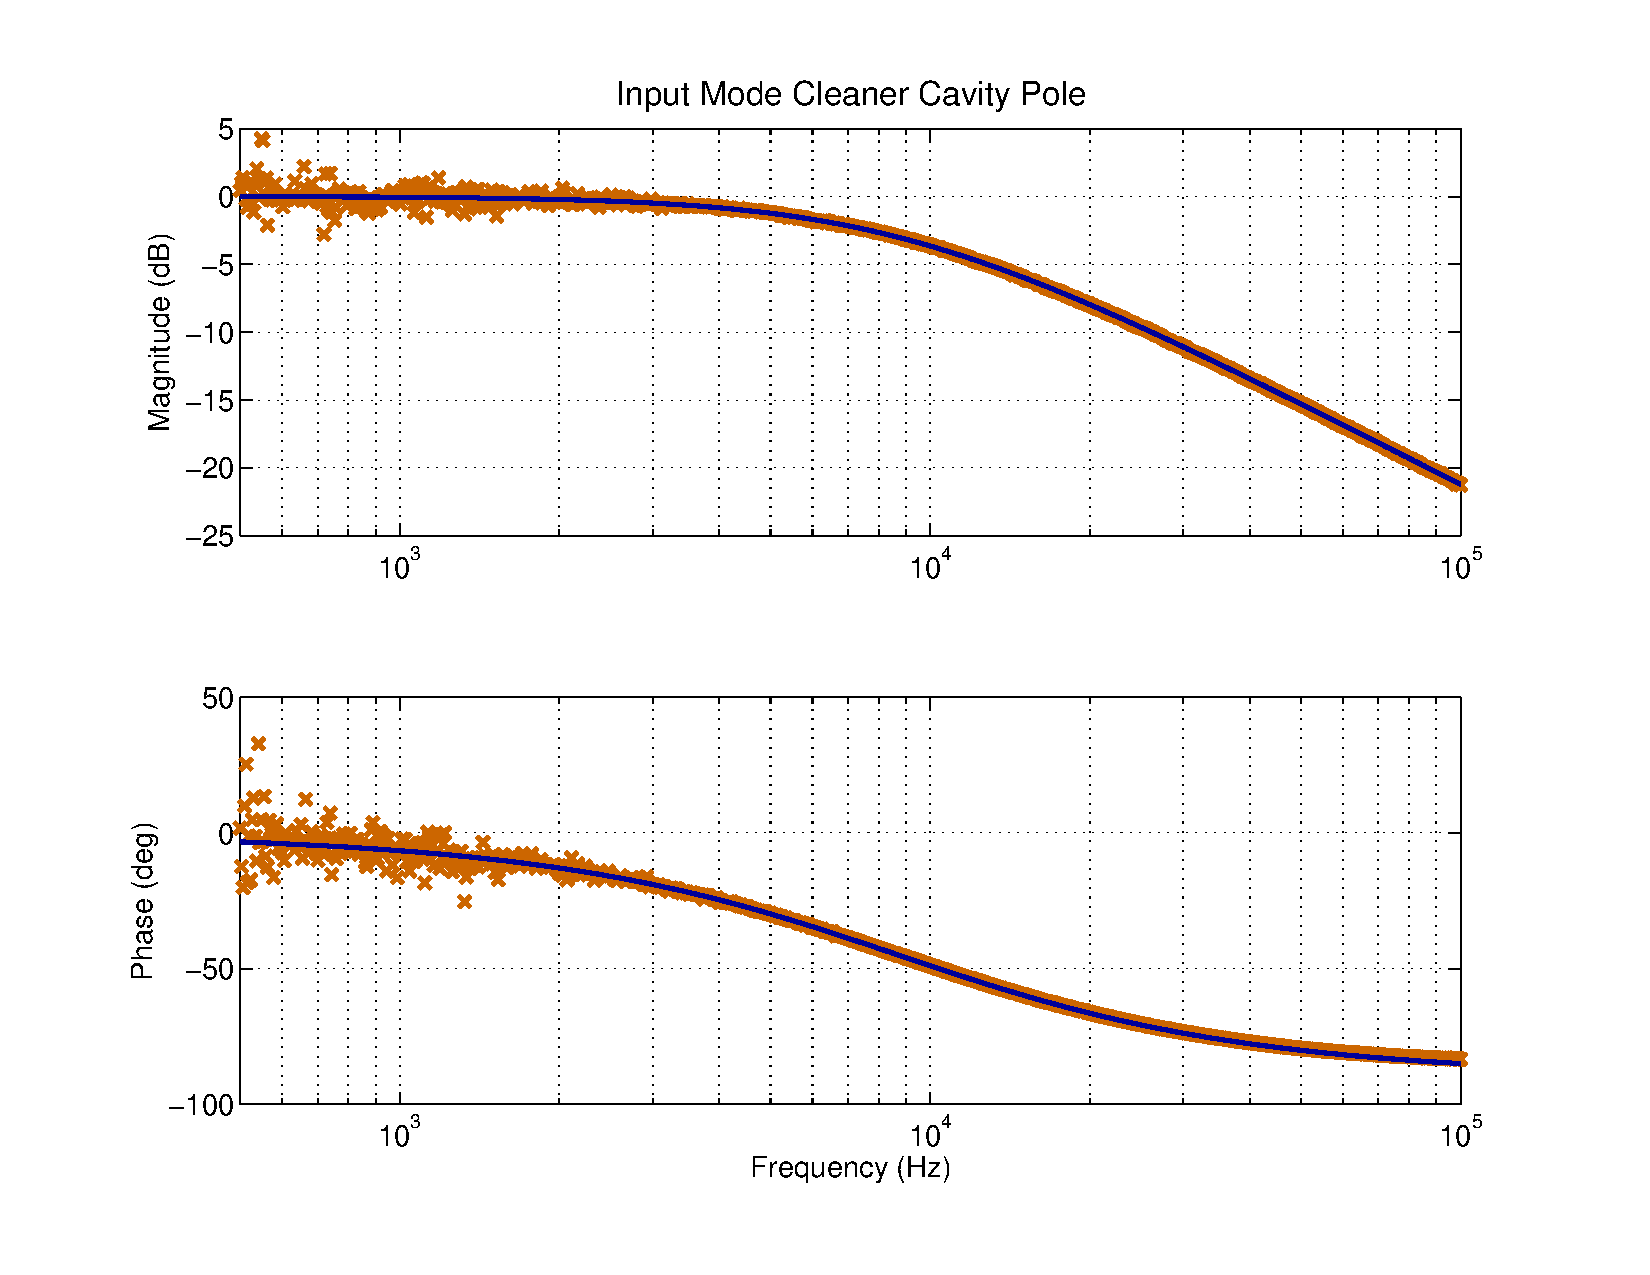
\includegraphics[width = 0.7\textwidth, trim = 2.5cm 1.5cm 2.5cm 1cm]{Cavity_Pole.pdf}
	\caption{The measured IMC cavity pole is shown together with a fit 
		to \eqref{eq:PoleApx}.  The fit has a pole frequency of 8712 Hz 
		which gives a finesse of 522.  These values are within the error 
		bars on the measured mirror reflectivities eliminating the 
		possibility of excessive losses.}
	\label{fig:cavPole}
\end{figure}

The results are shown in figure \ref{fig:cavPole} together with a fit to equation 
\eqref{eq:PoleApx}.  The results give a cavity pole of 8712 Hz which is equivalent 
to a finesse of 522.  
These numbers are exactly what was expected within the error bars of the measured 
reflectivity of the mirrors.  

%--------------------------------------------------------------------------------------------------
\subsection{Noise Budget}

As with all lock-in experiments, the measured feedback signals to the length and 
frequency path are a measure of the sensitivity of the input mode cleaner to length 
fluctuations.  
It is important to understand the source of this noise in the cavity measurement because 
some noise sources are quieted by feedback system while some noises, e.g. sensing noises, 
are impressed by the control system and show up
as frequency noise at the output of the input mode cleaner.  

Figure \ref{fig:NoiseBudget} shows the results of our efforts to understand the source 
of the measured length noise.  
There are two dominant terms which explain the length noise at low frequencies; 
seismic noise and damping sensor noise.  
Seismic noise dominates the low frequency noise but is filtered very steeply above the 
three suspension resonances.  
Damping sensor noise is length noise from the shadow sensors used for active damping
\textbf{Cite Earlier Section} being impressed onto the suspension through the damping loops.  

At higher frequencies, above 100 Hz, the measured noise is dominated by vibration s
of the injection bench of the prestabilized laser.  
The fact that this noise does not perfectly line up with the measured noise is due 
to the fact that the vibration noise is only measured at one point on the PSL table 
and the exact coupling is unknown.  


\begin{figure}[htb]
	\centering
	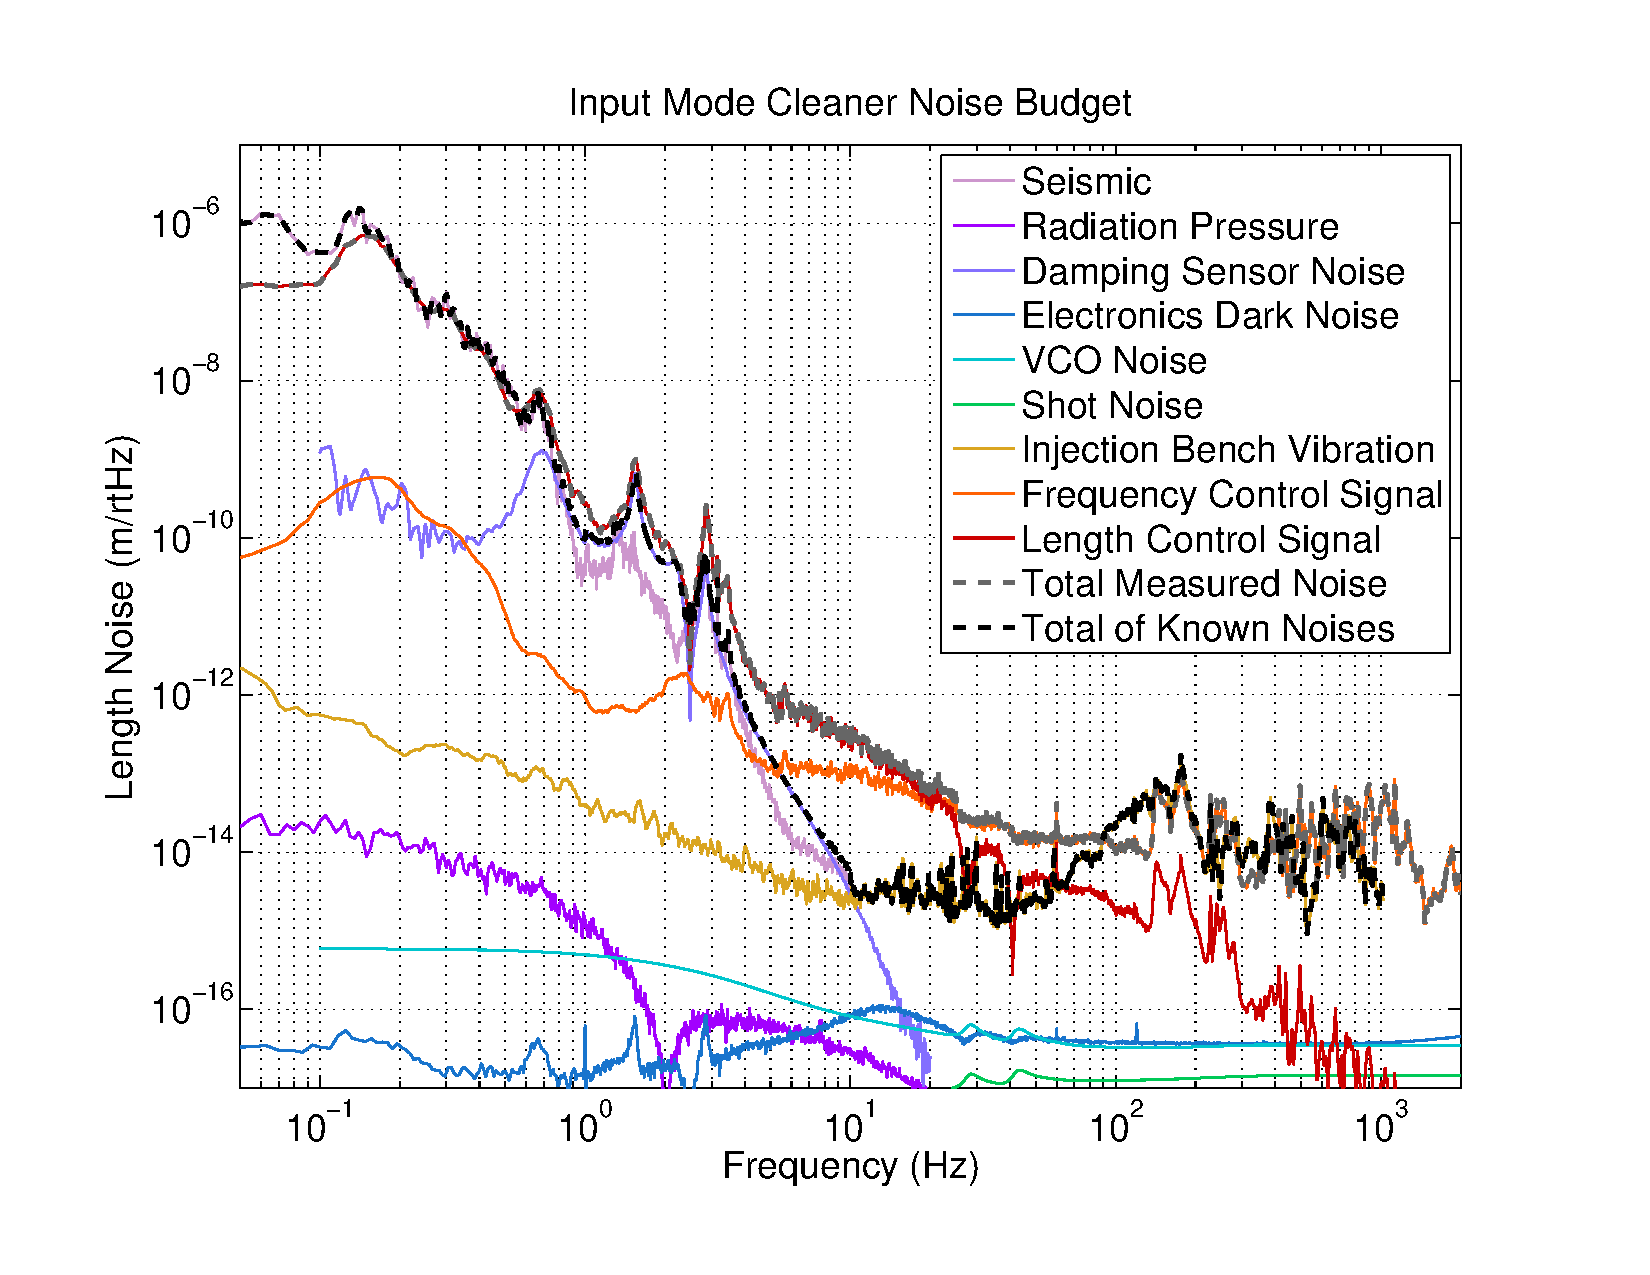
\includegraphics[width = 0.8\textwidth,trim = 2.5cm 1.5cm 2.5cm 1.5cm]{IMC_Noise_Budget.pdf}
	\caption{A noise budget for the input mode cleaner showing the measured control 
		signals together with the know noise sources.  Known noise sources explain 
		well the measured noise except for the gap between 5 Hz and 80 Hz.}
	\label{fig:NoiseBudget}
\end{figure}

%--------------------------------------------------------------------------------------------------
\subsection{Absorption Measurements}
The absorption in the input mode cleaner can be measured independently of the losses 
by tracking thermally sensitive properties of the mirrors.  
In this case we tracked two different thermally sensitive properties; 
the shift in the local radius of curvature of the optic 
and the shift in the frequency of the fundamental mechanical eigenmode of the mirror.  

The shift in the local radius of curvature of the optic was tracked by 
tracking the higher order mode spacing as a function of power.  
The spacing of the different higher order modes is dependent on the q 
parameter of the cavity which is itself dependent on the local radius of 
curvature of the mirrors.  
The Winkler et. al.\cite{Winkler1991} approximation for the local radius of 
curvature change is
\begin{equation}
	\frac{1}{\delta R}=\delta p=\frac{\alpha}{2\pi\omega^2\kappa}P_a,
\end{equation}
where $\alpha$ is the coefficient of thermal expansion of the mirror,  
$\kappa$ is the thermal conductivity, $\omega$ is the beam size, and 
$P_a$ is the power absorbed by the mirror.  
Assuming that the absorption is uniform across the mirrors and the same for 
each mirror ray matrix methods can be used to derive the Gouy phase shift 
of the cavity as a function of power.  
This Gouy phase shift can be expressed equivalently as the shift in the 
frequency location of the 10 peak.  
With these assumptions and approximations the shift in the location of the 10 
peak is given by 
\begin{equation}
	\delta f_{10}=-135.1 \frac{Hz}{ppm\cdot W},
\end{equation}
where the units of ppm is per mirror rather than total.

One of the difficulties with tracking the local radius of curvature change of 
the optics is that it is only sensitive to the total absorption and does not 
allow one to distinguish between mirrors.  
Tracking the fundamental mechanical eigenmode of the mirrors is however sensitive 
to the absorption of each mirror.  

The frequency of each of the three mirrors eigenmodes was first identified by 
driving the mirror around the frequency expected from FEA simulations.  
The feedback signal to the laser frequency was used as the readout mechanism.  
Figure \ref{fig:ModeTracking} shows the results of tracking the drumhead eigenfrequency 
of each of the optics during a 120 W power step lasting 75 minutes.  
The slope of the MC1 and MC2 curves is 2.55 times greater than the slope of the 
MC3 curve.  

\begin{figure}
	\centering
	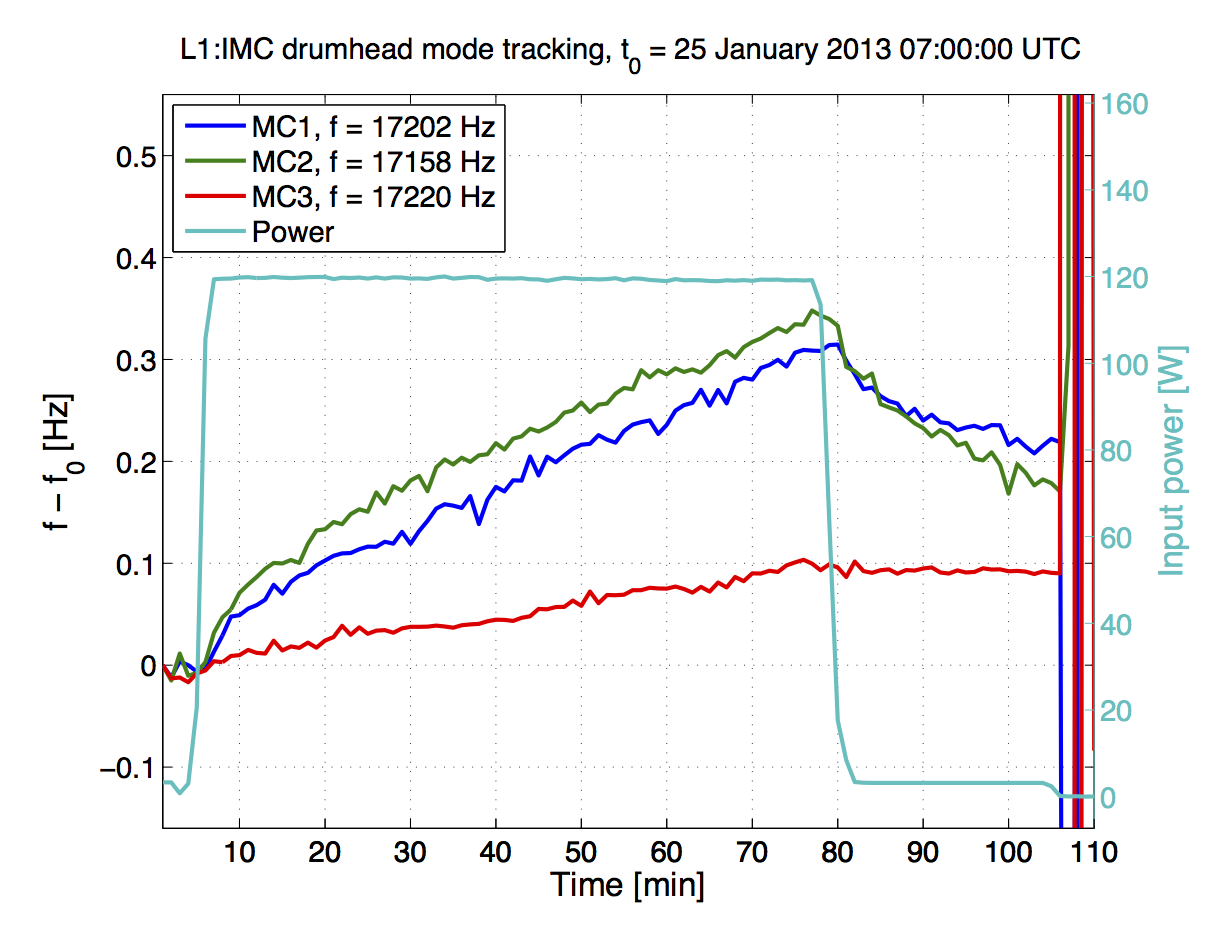
\includegraphics[width = 0.75\textwidth]{Mode_Tracking.png}
	\caption{The relative frequency shift of the drumhead eigenmodes of the input 
		mode cleaner optics is shown while the input power was increased to 120 W.  
		The slope of the increase is proportional to the absorption of the optic, 
		but turning the slope into an absolute number is heavily dependent on the 
		material parameters of the optics.  
		Combining the relative slopes with the higher order mode tracking measurement 
		allows for a precise determination of the absorption of each optic.}
	\label{fig:ModeTracking}
\end{figure}	

Including this relative slope information in the gouy phase shift calculation described 
above, the frequency shift of the 01 mode for MC3 is $\delta f_{MC3}=274.6\ \tfrac{Hz}{ppm*W}$ 
with MC1 and MC2 being a factor of 2.55 times lower.  
Putting all of this together gives the absorption numbers quoted in table \ref{tab:Absorption}.

\begin{table}
	\centering
	\begin{tabular}{|c||c|c|}
		\hhline{|--|-|}
		Optic & Absorption (ppm) & Error (ppm)\\
		\hhline{|=#=|=|}
		MC1 & 2.11 & 0.08 \\
		\hhline{|--|-|}
		MC2 & 2.11 & 0.08 \\
		\hhline{|--|-|}
		MC3 & 0.83 & 0.03 \\
		\hhline{|--|-|}
	\end{tabular}
	\caption{Measured absorption of the three optics of the input mode cleaner.  
		The relative absorption between the optics was measured with the eigenmode tracking 
		scheme and the total absorption was measured by tracking the higher order mode 
		frequency while changing the power.}
	\label{tab:Absorption}	
\end{table}	



%--------------------------------------------------------------------------------------------------
\subsection{Thermal Lensing}


\begin{thebibliography}{9}
	\bibitem{drawcite}
		Uses the vector components library developed by Alexander Franzen; available at http://www.gwoptics.org/ComponentLibrary/
	\bibitem{EricBlack}
		Eric Black's PDH paper.
	\bibitem{DreverHall}
		The Drever hall paper on the PDH technique.		
	\bibitem{Winkler1991}
		Winkler, W., K. Danzmann, A. Rudiger, and R. Schilling. Heating by Optical Absorption and 
		the Performance of Interferometric Gravitational-Wave Detectors." Phys. Rev. A 44 117022-7036. 1 December, 1991.
	\bibitem{Anderson1984}
		Anderson, Dana Z.  ``Alignment of Resonant Optical Cavities.''  Applied Optics.  
		Vol. 23 No. 17 1 September, 1984.
	\bibitem{Morrison1994}
		Morrison, E. et. al. ``Automatic Alignment of Optical Interferometers.''  Applied Optics.  
		Vol. 33 No. 22 1 August, 1994.
	\bibitem{Fritschel1998}
		Fritschel, P. et. al. ``Alignment of an Interferometric Gravitational Wave Detector.''  Applied Optics.  
		Vol. 37 No. 28 1 October, 1998.	
	\bibitem{Finesse}
		http://www.gwoptics.org/finesse/
	\bibitem{Arai2013}
		Arai, K. et. al. ``Finesse Simulation for the Alignment Control Signal of the aLIGO Input Mode 
		Cleaner.'' LIGO-T1300074-v1.
\end{thebibliography}		

\end{document}
